\documentclass[11pt]{article}
\usepackage{libertine}
\usepackage{tikz}

\title{{\em Modern Climate Change}: a cheat-sheet}
\begin{document}

\maketitle

\section{Introduction}
This doc is a collection of notes from the climate science chapters of the
book {\em Modern Climate Change} by Andrew Dessler. It's intended as a quick
reference for the main concepts and formulas for those who've read the book.

\section{Climate history}

\section{Radiation and energy balance}

\section{Simple climate models}
\[
T = \sqrt[4]{\frac{(n+1)S(1-\alpha)}{4 \sigma}}
\]


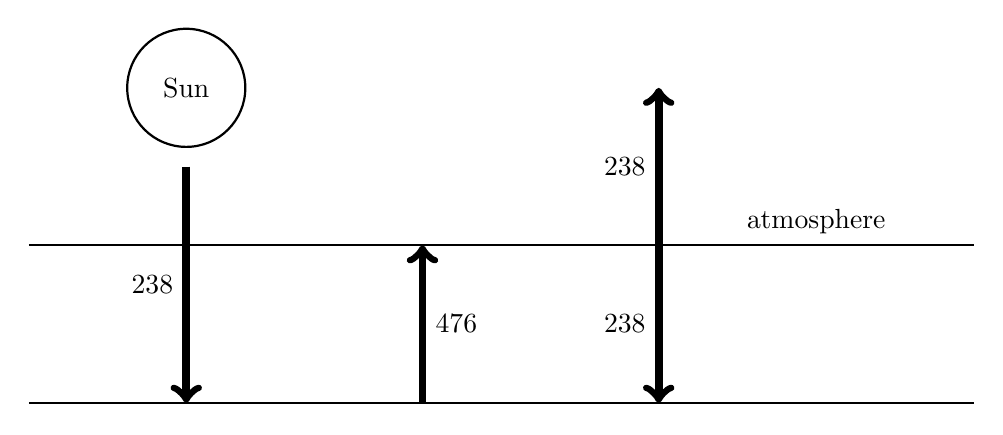
\begin{tikzpicture}[xscale=2]
    % Sun
    \node at (1,4) [circle, draw, thick, minimum size=1.5cm] {Sun};

    % Atmosphere layer
    \draw[thick] (0, 2) -- (6, 2);
    \node at (5, 2.3) {atmosphere};

    % Ground layer
    \draw[thick] (0, 0) -- (6, 0);

    % Arrows
    % sun to earth
    \draw[line width=1mm, ->] (1, 3) -- (1, 0) node[midway, left] {238};
    % earth to atmosphere
    \draw[line width=1mm, ->] (2.5, 0) -- (2.5, 2) node[midway, right] {476};

    % atmosphere to earth
    \draw[line width=1mm, ->] (4, 2) -- (4, 0) node[midway, left] {238};
    % atmosphere to space   
    \draw[line width=1mm, ->] (4, 2) -- (4, 4) node[midway, left] {238};

\end{tikzpicture}

\section{The carbon cycle}
\section{Forcings, feedbacks, and climate sensitivity}

\end{document}